\begin{figure}
\begin{subfigure}{0.45\textwidth}
\centering
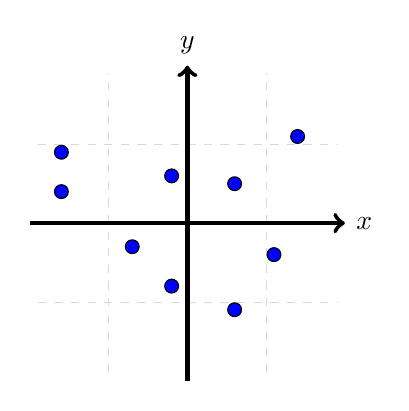
\begin{tikzpicture}
    \draw[help lines, color=gray!30, dashed] (-1.9,-1.9) grid (1.9,1.9);
    \draw[->,ultra thick] (-2,0)--(2,0) node[right]{$x$};
    \draw[->,ultra thick] (0,-2)--(0,2) node[above]{$y$};

        \node[draw, circle, fill=blue, inner sep=0pt, minimum size=5pt] (p1) at (-1.6, 0.4) {};
        \node[draw, circle, fill=blue, inner sep=0pt, minimum size=5pt] (p2) at (-1.6, 0.9) {};
        \node[draw, circle, fill=blue, inner sep=0pt, minimum size=5pt] (p3) at (-0.7, -0.3) {};
        \node[draw, circle, fill=blue, inner sep=0pt, minimum size=5pt] (p4) at (-0.2, 0.6) {};
        \node[draw, circle, fill=blue, inner sep=0pt, minimum size=5pt] (p5) at (-0.2, -0.8) {};
        \node[draw, circle, fill=blue, inner sep=0pt, minimum size=5pt] (p6) at (0.6, 0.5) {};
        \node[draw, circle, fill=blue, inner sep=0pt, minimum size=5pt] (p7) at (1.1, -0.4) {};
        \node[draw, circle, fill=blue, inner sep=0pt, minimum size=5pt] (p8) at (1.4, 1.1) {};
        \node[draw, circle, fill=blue, inner sep=0pt, minimum size=5pt] (p9) at (0.6, -1.1) {};

\end{tikzpicture}
\caption{The original list of points.}\label{fig:symmetry-breaking-1}
\end{subfigure}
\begin{subfigure}{0.45\textwidth}
    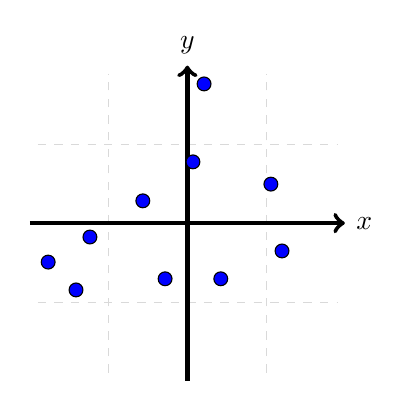
\begin{tikzpicture}
        \draw[help lines, color=gray!30, dashed] (-1.9,-1.9) grid (1.9,1.9);
        \draw[->,ultra thick] (-2,0)--(2,0) node[right]{$x$};
        \draw[->,ultra thick] (0,-2)--(0,2) node[above]{$y$};
    
        \node[draw, circle, fill=blue, inner sep=0pt, minimum size=5pt] (p1) at (-1.4142137010204086, -0.8485279063449582) {};
        \node[draw, circle, fill=blue, inner sep=0pt, minimum size=5pt] (p2) at (-1.7677670338439557, -0.4949744579819674) {};
        \node[draw, circle, fill=blue, inner sep=0pt, minimum size=5pt] (p3) at (-0.2828428280140589, -0.7071067349707606) {};
        \node[draw, circle, fill=blue, inner sep=0pt, minimum size=5pt] (p4) at (-1.2374368959613027, -0.176776493102608) {};
        \node[draw, circle, fill=blue, inner sep=0pt, minimum size=5pt] (p5) at (-0.5656853787334529, 0.2828428049061702) {};
        \node[draw, circle, fill=blue, inner sep=0pt, minimum size=5pt] (p6) at (0.4242639531724791, -0.7071068505102043) {};
        \node[draw, circle, fill=blue, inner sep=0pt, minimum size=5pt] (p7) at (0.07071080521204193, 0.7778174477512475) {};
        \node[draw, circle, fill=blue, inner sep=0pt, minimum size=5pt] (p8) at (1.0606602526574178, 0.4949745735214111) {};
        \node[draw, circle, fill=blue, inner sep=0pt, minimum size=5pt] (p9) at (0.21213232320457065, 1.767766918304512) {};
        \node[draw, circle, fill=blue, inner sep=0pt, minimum size=5pt] (p10) at (1.202081470247393, -0.3535535870103234) {};
    \end{tikzpicture}

\caption{After rotating by $45^\circ$ all points have different $x$ coordinates.}\label{fig:symmetry-breaking-2}
\end{subfigure}

\vspace{0.5cm}

\begin{subfigure}{0.48\textwidth}
    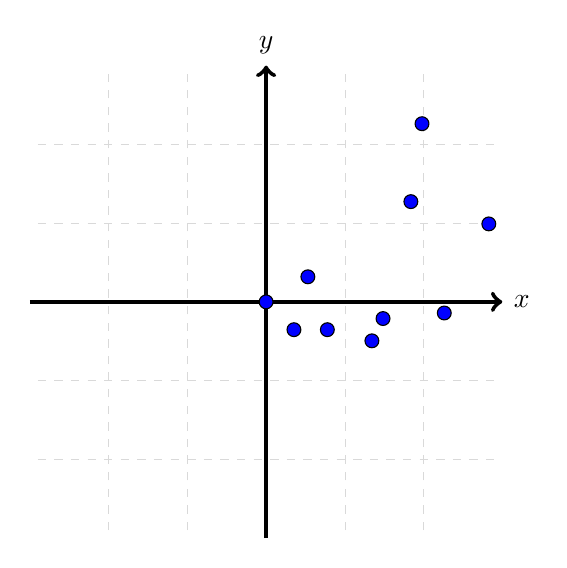
\begin{tikzpicture}
        \draw[help lines, color=gray!30, dashed] (-2.9,-2.9) grid (2.9,2.9);
        \draw[->,ultra thick] (-3,0)--(3,0) node[right]{$x$};
        \draw[->,ultra thick] (0,-3)--(0,3) node[above]{$y$};
    
        \node[draw, circle, fill=blue, inner sep=0pt, minimum size=5pt] (p1) at (0.3535533328235472, -0.35355344836299085) {};
        \node[draw, circle, fill=blue, inner sep=0pt, minimum size=5pt] (p2) at (0.0, 0.0) {};
        \node[draw, circle, fill=blue, inner sep=0pt, minimum size=5pt] (p3) at (1.3435028033768117, -0.49497496635551974) {};
        \node[draw, circle, fill=blue, inner sep=0pt, minimum size=5pt] (p4) at (0.530330137882653, 0.31819796487935936) {};
        \node[draw, circle, fill=blue, inner sep=0pt, minimum size=5pt] (p5) at (0.7778174015354699, -0.3535535176866571) {};
        \node[draw, circle, fill=blue, inner sep=0pt, minimum size=5pt] (p6) at (1.4849242058298968, -0.21213227698879322) {};
        \node[draw, circle, fill=blue, inner sep=0pt, minimum size=5pt] (p7) at (2.262741676689033, -0.14142172596352753) {};
        \node[draw, circle, fill=blue, inner sep=0pt, minimum size=5pt] (p8) at (1.8384778390559977, 1.2727919057332149) {};
        \node[draw, circle, fill=blue, inner sep=0pt, minimum size=5pt] (p9) at (2.8284272865013733, 0.9899490315033785) {};
        \node[draw, circle, fill=blue, inner sep=0pt, minimum size=5pt] (p10) at (1.9798993570485264, 2.2627413762864794) {};
    \end{tikzpicture}

\caption{After translating the leftmost point is at $(0,0)$.}\label{fig:symmetry-breaking-3}
\end{subfigure}
\begin{subfigure}{0.45\textwidth}
    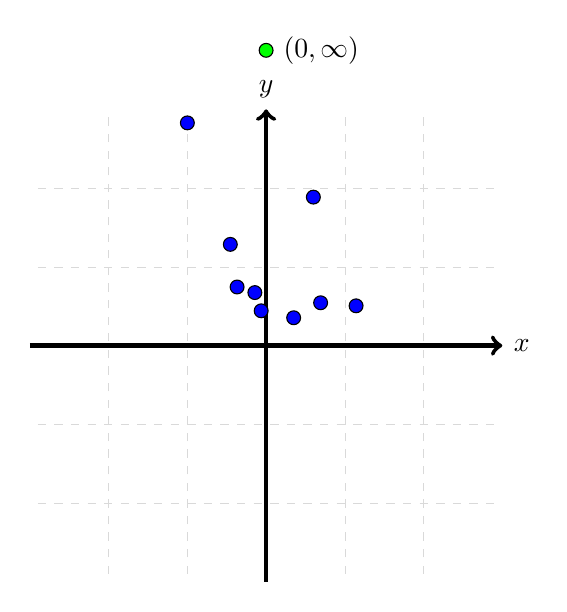
\begin{tikzpicture}
        \draw[help lines, color=gray!30, dashed] (-2.9,-2.9) grid (2.9,2.9);
        \draw[->,ultra thick] (-3,0)--(3,0) node[right]{$x$};
        \draw[->,ultra thick] (0,-3)--(0,3) node[above]{$y$};
    
        \node[draw, circle, fill=blue, inner sep=0pt, minimum size=5pt] (p1) at (-1.0000003267949498, 2.8284275869040783) {};
        \node[draw, circle, fill=blue, inner sep=0pt, minimum size=5pt] (p2) at (-0.36842123820763945, 0.74432297237234) {};
        \node[draw, circle, fill=blue, inner sep=0pt, minimum size=5pt] (p3) at (0.5999997777794923, 1.8856178983010607) {};
        \node[draw, circle, fill=blue, inner sep=0pt, minimum size=5pt] (p4) at (-0.45454565170272093, 1.285648788553618) {};
        \node[draw, circle, fill=blue, inner sep=0pt, minimum size=5pt] (p5) at (-0.14285730958923684, 0.6734350454211354) {};
        \node[draw, circle, fill=blue, inner sep=0pt, minimum size=5pt] (p6) at (-0.06250016403572127, 0.4419417427548577) {};
        \node[draw, circle, fill=blue, inner sep=0pt, minimum size=5pt] (p7) at (0.692307450595518, 0.5439282316905542) {};
        \node[draw, circle, fill=blue, inner sep=0pt, minimum size=5pt] (p8) at (0.34999981658637486, 0.353553370373877) {};
        \node[draw, circle, fill=blue, inner sep=0pt, minimum size=5pt] (p9) at (1.1428567660426896, 0.5050761779582166) {};

        \node[draw, circle, fill=green, inner sep=0pt, minimum size=5pt, label={[xshift=0.7cm, yshift=-0.4cm]$(0, \infty)$}] (p10) at (0, 3.75) {}; 
    \end{tikzpicture}

\caption{}\label{fig:symmetry-breaking-4}
\end{subfigure}


\begin{subfigure}{0.45\textwidth}


\caption{}\label{fig:symmetry-breaking-3}
\end{subfigure}
\begin{subfigure}{0.45\textwidth}


\caption{}\label{fig:symmetry-breaking-4}
\end{subfigure}



\caption{Illustration of the proof of the main symmetry breaking theorem.}\label{fig:symmetry-breaking}
\end{figure}